\section{History of CNN's}
CNNs are a special kind of architecture that was popularised in the 2010s.
It is vabuely based on biological processes and visual cortexes from biology.
These kinds of networks is most commonly applied to visual imagery. 
They are also applicable to other kinds of data. A simple rule of thumb 
is that data where if swapping columns of the data matrix removes the 
information contained in the data, convolutional neural networks may be used.

\section{Convolution Layer}

\begin{figure}[H]
    \centering
    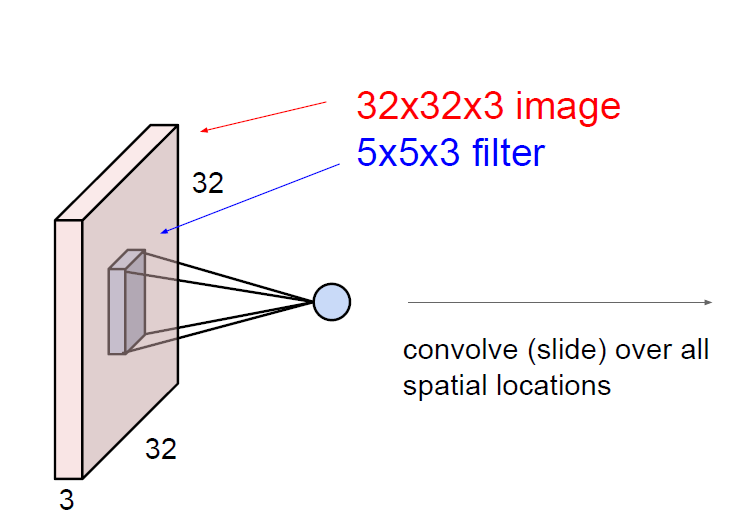
\includegraphics[width=0.5\linewidth]{figures/convolution.PNG}
    \caption{Convolution layer}
\end{figure}

The central concept of CNNs (it is even in its name) is the convolution. 
A convolution can be though of as passing a filter or kernel through the image
to average it out. The selection of kernel determines what visual features is 
extracted from the image. Using multiple filters to get different features
is not uncommon.

\medskip

In many convolutional neural networks found in publications. These typically are
very deep, has many different convolutions and pooling layers and ending in a 
fully connected layer which. The layers before the fully connected layer 
is there for simply extracting features and preprocessing the data. The fully 
connected layer is there for inference.

\medskip

It is not uncommon to use existing CNN architectures from publications and
remove the fully connected layer at the end to suit it for your own needs.
In those cases one assume that the existing CNN architecture is able to collect
high quality features for ones problem. This saves time on training the
CNN part of the network and one can focus on training the inference layer at the
end.

\begin{figure}[H]
    \centering
    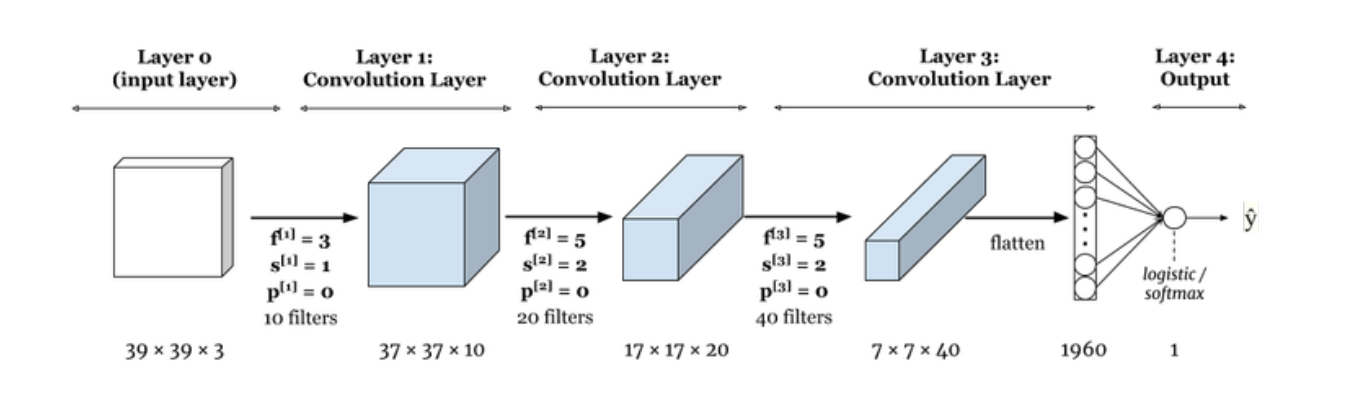
\includegraphics[width=\linewidth]{figures/CNN.PNG}
    \caption{CNN architecture}
\end{figure}

\section{Number of weights after convolution layers}

When working with CNNs and Neural Networks in general it is regular to talk
about parameters. Parameters are weights in the neural network and is learned
through backpropagation. Below is a list of the different layers and their
parameters. The numbers and calculations are examples.

\subsection{Size of output tensorf for a conv layer}

Let us define

\begin{gather*}
    O = \text{Size (width) of output image} \\
    I = \text{Size (width) of input inage} \\
    K = \text{Size (width) of the kernels used in conv layer} \\
    N = \text{Number of kernels} \\
    S = \text{Stride of the conv layer} \\
    P = \text{Padding} \\
\end{gather*}

The size $O$ is given Bayes

\begin{equation}
    O = \frac{I - K + 2P}{S} + 1
\end{equation}

\textbf{Example:} Let's say we have a image of size $32 \times 32 \times 3$,
 $5$ kernels $5 \times 5 \times 3$, stride $1$ and padding $0$ we get

\begin{equation*}
    O = \frac{32 - 5 - 0}{1} + 1 = 28
\end{equation*}

the image is then $28 \times 28 \times 5$

\subsection{Size of output of maxpool layer}

\begin{gather*}
    O = \text{Size (width) of output image} \\
    I = \text{Size (width) of input inage} \\
    S = \text{Stride of the convolution operation} \\
    P = \text{Pool size}
\end{gather*}

The output size $O$ is then given by 

\begin{equation*}
    O = \frac{I - P}{S} + 1
\end{equation*}

\subsection{Number of parameters in a Conv layer}

\begin{gather*}
    B = \text{Number of biases in conv layer} \\
    P = \text{Number of parameters of conv layer} \\
    K = \text{Size of kernels used in conv layer} \\
    N = \text{Number of kernels} \\
    C = \text{Numberof channels of the input image} \\
\end{gather*}

The parameters is then calculated as

\begin{equation*}
    P = (K^2 \times C \times N) + B
\end{equation*}

Note: $B = N$ 

\textbf{Example:} Assume that we have the same kernels as above then we get
$P = 28^2 \times 3 \times 5 + 5 = 380$


